\documentclass[11pt]{article}
\usepackage{fullpage}
\usepackage{listings}
\usepackage{needspace}
\usepackage{color}
\usepackage{ifthen}
\usepackage{pgf}
\usepackage{tikz}
\usetikzlibrary{arrows,automata}
\usepackage{amsmath}

\lstset{ %
basicstyle=\footnotesize,       % the size of the fonts that are used for the code
numbers=left,                   % where to put the line-numbers
stepnumber=1,                   % the step between two line-numbers. If it's 1 each line will be numbered
numbersep=5pt,                  % how far the line-numbers are from the code
showspaces=false,               % show spaces adding particular underscores
showstringspaces=false,         % underline spaces within strings
tabsize=4,		                % sets default tabsize to 4 spaces
language=Python
}

\ifthenelse{\isundefined{\isAnswerKey}}
{
    \newenvironment{answer}{\large\lstset{basicstyle=\large}\color{white}}{}
}
{
    \newenvironment{answer}{\large\lstset{basicstyle=\large}\color{red}}{}
}


\author{Computer Science Community}
\title{CS-242 Final Exam Review}
\date{Winter, 2011-2}

\makeatletter
\let\thetitle\@title
\let\theauthor\@author
\let\thedate\@date
\makeatother

\begin{document}
\noindent{\Large \thetitle \hfill \thedate}

\begin{enumerate}

\item How can you use a stack to determine if an input string has properly
      balanced parens, brackets and braces. (eg. ``[\{\}]'' is accepted, but
      ``(()'' and ``[(])'' are not)?

    \begin{answer}
    \begin{lstlisting} 
def delims_are_balanced(inString):
    ''' String -> boolean
    Determines if the input string has balanced delimiters
    Delimiters are () [] {} and <>  
    
    '''
    delim = {'(': ')', '[': ']', '{': '}', '<': '>'}
    stack = Stack()
    for char in inString:
        if char in delim:
            stack.push(char)
        elif char in delim.values():
            if stack.is_empty():
                return False
            if delim[stack.peek()] == char:
                stack.pop()
            else:
                return False
    return stack.is_empty()
    \end{lstlisting}
    \end{answer}

\item What role does the queue play in a Breadth First Search?

    \begin{answer}
    The FIFO nature of a queue ensures that vertices are visited on a level-by-level basis. That is, if the traversal 
    begins at vertex $v$, then all of $v$'s children are visited, followed by $v$'s grandchildren and so on. It is
    this behavior that ensures that the path selected from a start vertex to a end vertex is of minimal length.
    \end{answer}

\item Given a Breadth First Search algorithm, how would you change it to
      perform a Depth First Search?

    \begin{answer}
    Change the queue to a stack.
    \end{answer}

\item What data structures can be used to represent a weighted  digraph? How?

    \begin{answer}
    A matrix, a hash table and a linked structure.
    {\bf With a matrix}, we can create a table such that the element at W[a][b]
    contains edge weight between two nodes. This approach works well for dense
    graphs.
    {\bf With a hash table}, we can key on the source node and store a list of
    attached nodes, along with their weights. This approach works well for
    sparse graphs, because it uses less memory than a matrix.
    We also have the option of using a {\bf purely linked structure}, such that
    each node has a list of other nodes that it connects to, with an associated
    cost. This will most closely resemble the actual structure of the graph in
    memory, but it may become difficult to manage.
    \end{answer}

\item When is a vertex's sum weight finalized in Dijkstra's algorithm?

    \begin{answer}
    A vertex's sum weight is final after it has updated the tentative distances
    of all of its neighbors. As part of being finalized, it's moved from the
    unvisited set to the visited set.
    \end{answer}

\item What role does the priority queue play in finding the shortest path?
      When do we use it?

    \begin{answer}
    The priority queue is used to select the next vertex to visit. We want to
    visit the node which currently has the lowest tentative distance from the
    start, so we use a priority queue which always returns the lowest element.
    \end{answer}

\item Why does Dijkstra's algorithm not work correctly on graphs with negative
      edge weights?

    \begin{answer}
    Dijkstra's algorithm doesn't work correctly on graphs with negative edge
    weights due to one of its {\em greedy} behaviors.

    When selecting the next node to visit, Dijkstra's algorithm chooses the
    node with the current lowest total value, then {\em finalizes} that value
    forever. If there were another route to that node, which had not yet been
    explored (and contained a net negative weight) Dijkstra's algorithm would
    return a suboptimal path. In the following example, the final transitive
    costs should be \{A:0,B:1,C:3\} but Dijkstra's algorithm produces
    \{A:0,B:2,C:3\}.

    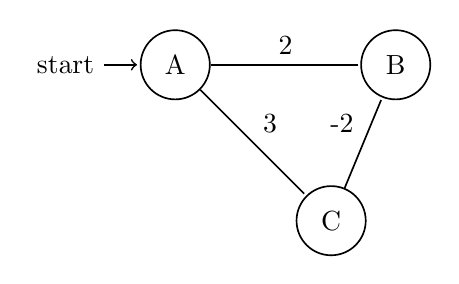
\begin{tikzpicture}[shorten >=1pt,auto,node distance=2.8cm,semithick]
        \node[initial,state] (A) {A};
        \node[state]        (B) [right of=A] {B};
        \node[state]        (C) [below right of=A] {C};

        \path   (A) edge node {2} (B)
                    edge node {3} (C)
                (C) edge node {-2} (B);
    \end{tikzpicture}
    \end{answer}

\section*{Backtracking}

\item How is backtracking better suited for solving a Tetravex board than
      using regular brute force?

    \begin{answer}
    \Huge TODO: Write answer
    \end{answer}

\pagebreak
\section*{Hashing and Hash Tables}

\item Chris made a mistake in his chaining implementation!

\begin{lstlisting}
def noobDictionaryChaining():

    emptyList = []
    d = [emptyList for x in range(3)]

    d[hash('curling')].append['curling']
    d[hash('is')].append['is']
    d[hash('cool')].append['cool']
    d[hash('now')].append['now']
    print(d)
\end{lstlisting}

    \begin{enumerate}
    \item Show what the dictionary (hashtable) looks like after this function
          completes. Assume the hash() function returns len(input) \% len(d).

        \begin{answer}
        All of the elements in the hash table are a reference to the same list,
        so all lookups will take $O(n)$ time.
        \vspace{2in}
        \end{answer}

    \item What can we do to make the function behave as Chris expects it to
          behave?

        \begin{answer}
        Line 6 should be ``d[i] = []''.
        \end{answer}

    \item Draw the table of the properly behaving hash function.
        
        \begin{answer}
        \vspace{3.5in}
        \end{answer}
    \end{enumerate}


\section*{Sorting}

\item Fill in the table for the asymptotic running time of each sorting
      algorithm.
      \begin{center}
      \begin{tabular}{|r|c|c|c|}
        \hline
        ~ & Best & Worst & Average \\\hline
        MergeSort &
            \begin{answer}$O(n*\textrm{log}(n))$\end{answer} &
            \begin{answer}$O(n*\textrm{log}(n))$\end{answer} &
            \begin{answer}$O(n*\textrm{log}(n))$\end{answer} \\\hline
        Quicksort &
            \begin{answer}$O(n*\textrm{log}(n))$\end{answer} &
            \begin{answer}$O(n^2)$\end{answer} &
            \begin{answer}$O(n*\textrm{log}(n))$\end{answer} \\\hline
        HeapSort &
            \begin{answer}$O(n*\textrm{log}(n))$\end{answer} &
            \begin{answer}$O(n*\textrm{log}(n))$\end{answer} &
            \begin{answer}$O(n*\textrm{log}(n))$\end{answer} \\\hline
      \end{tabular}
      \end{center}

\item What sorting algorithm splits its input list into two other lists, one
      which has element which are all smaller than a value (which is randomly
      selected) and one which has elements which are all larger than the
      randomly selected value?

    \begin{answer}
    Quicksort.
    \end{answer}

\item\label{qsort-worst-case} What kind of data causes Quicksort's worst-case
      time complexity? You may assume that we always pick the first element as
      the pivot.

      \begin{answer}
      Data that is (nearly) sorted or is sorted in reverse order.
      \end{answer}

\item What causes Quicksort to run so slowly on the input you describe in
      question \ref{qsort-worst-case}?

    \begin{answer}
    Quicksort splits its input into two lists based on the value of the pivot.
    If the pivot is either the smallest or the largest element, then one list
    will only have no elements, while the others will have all of the elements
    but the pivot. We can see this if we perform a substitution trace:

\begin{verbatim}
qsort([1,2,3,4])
qsort([]) + [1] + qsort([2,3,4])
qsort([]) + [1] + qsort([]) + [2] + qsort([3,4])
qsort([]) + [1] + qsort([]) + [2] + qsort([]) + [3] + qsort([4])
qsort([]) + [1] + qsort([]) + [2] + qsort([]) + [3] + qsort([4])
qsort([]) + [1] + qsort([]) + [2] + qsort([]) + [3] + qsort([]) + [4] + qsort([])
[1,2,3,4]
\end{verbatim}
    \end{answer}

\item In Quicksort, why do we select a random pivot value, rather than always
      pivoting on the first element?

      \begin{answer}
      With real-world data, we're more likely to encounter ordered or
      semi-ordered data than randomised data. This makes it more likely for us
      run into Quicksort's worst-case time complexity. We run into this bad
      time complexity if we select pivots which are near the lowest or highest
      values.

      Selecting a random value to pivot on helps us encounter the average case
      evens out the distribution of ordered and unordered data. Even if we're
      getting in sorted data, if we select pivots randomly, we should be able
      to end up with average time complexity.
      \end{answer}

\item Show the stages of a Merge sort and a Quicksort on the following list:
      [3,5,1,3,2,7,9]. Be sure to identify your pivot.

    \begin{answer}
    \Huge TODO
    \end{answer}

\section*{Heaps and Heapsort}

\item For a binary heap containing $n$ elements, what is the maximum number of
      swaps occurring after an insert operation?

    \begin{answer}
    \Huge TODO
    \end{answer}

\item Given a node in an array-based binary heap at index $i$, where are the
      indices of both its children? What is the index of its parent?

    \begin{answer}
    The children are at $2i+1$ and $2i+2$. The parent is at
    $\lfloor\frac{i-1}{2}\rfloor$.

    \marginpar{\small\em Note that in a 1 indexed array system, the children
    would be at $2i$ and $2i+1$. The parent would be at
    $\lfloor\frac{i}{2}\rfloor$.}
    \end{answer}

\item Run a heap sort on the following list: [3,5,1,3,2,7,9], showing the heap
      at each stage. Be sure to heapify the list first.

    \begin{answer}
    \vspace{3.5in}
    \end{answer}

\section*{Dynamic Programming}

\item When we trace all of the function calls being made while computing the
      n'th number in the Fibonacci sequence from a solution given earlier in
      the quarter, we notice that there is a lot of extra work being done.

      \marginpar{\small\em You can safely ignore the things mentioning
      `ftrace': those are just there to make drawing the call graph easy.}
      \lstinputlisting{naive_fibonacci.py}

\begin{verbatim}
>>> fib(4)
    0 fib( (4,) {} )
    1 |  fib( (3,) {} )
    2 |  |  fib( (2,) {} )
    3 |  |  |  fib( (1,) {} )               # fib(1) called
    3 |  |  |  fib( (1,) {} ) returns: 1
    3 |  |  |  fib( (0,) {} )
    3 |  |  |  fib( (0,) {} ) returns: 0
    2 |  |  fib( (2,) {} ) returns: 1
    2 |  |  fib( (1,) {} )                  # fib(1) called again
    2 |  |  fib( (1,) {} ) returns: 1
    1 |  fib( (3,) {} ) returns: 2
    1 |  fib( (2,) {} )
    2 |  |  fib( (1,) {} )                  # fib(1) called once more
    2 |  |  fib( (1,) {} ) returns: 1
    2 |  |  fib( (0,) {} )
    2 |  |  fib( (0,) {} ) returns: 0
    1 |  fib( (2,) {} ) returns: 1
    0 fib( (4,) {} ) returns: 3
\end{verbatim}

      Write a dynamic programming implementation of `fib' which will not do
      duplicate work.

    \begin{answer}
    \marginpar{\small\em Note the approach to default assignment for the table:
    if table was set to [0,1] in the parameter list, we would be modifying it
    globally whenever we appended to it.}
    \lstinputlisting{memoized_fibonacci.py}
\begin{verbatim}
>>> fib(4)
    0 fib( (4,) {} )
    1 |  fib( (3, [0, 1]) {} )
    2 |  |  fib( (2, [0, 1]) {} )
    3 |  |  |  fib( (1, [0, 1]) {} )
    3 |  |  |  fib( (1, [0, 1]) {} ) returns: 1
    3 |  |  |  fib( (0, [0, 1]) {} )
    3 |  |  |  fib( (0, [0, 1]) {} ) returns: 0
    2 |  |  fib( (2, [0, 1]) {} ) returns: 1
    2 |  |  fib( (1, [0, 1, 1]) {} )
    2 |  |  fib( (1, [0, 1, 1]) {} ) returns: 1
    1 |  fib( (3, [0, 1]) {} ) returns: 2
    1 |  fib( (2, [0, 1, 1, 2]) {} )
    1 |  fib( (2, [0, 1, 1, 2]) {} ) returns: 1
    0 fib( (4,) {} ) returns: 3
\end{verbatim}
    \end{answer}

\end{enumerate}

\end{document}
